% ----------------------------------------------------------------
% Revisão bibliográfica *******************
% ----------------------------------------------------------------
\chapter{Desenvolvimento}
\label{cap:desenvolvimento}
%
%
O desenvolvimento da \textit{SAGA Game Library} ou SGL, assim como todo \textit{software}, passou por diversas etapas para que no final torna-se possível obter um produto condizente com a proposta do trabalho.
\par 
O desenvolvimento de um \textit{software}, de maneira geral, sempre é composto das seguintes etapas:
%
\begin{itemize}
 \item Especificação dos requisitos do \textit{software}: Descrição do objetivo e do se espera do \textit{software}.
 \item Projeto do sistema: decisão dos conceitos relacionado ao que deve ser implementado, incluindo a escolha da linguagem de programação
 adequada, sistema operacional alvo, bibliotecas e ferramentas auxiliares.
 \item Implementação: O próprio desenvolvimento do \textit{software}. Consiste na transformação de todo conteúdo formulado na fase de projeto em código.
 \item Teste e depuração: Fase que consiste no teste do \textit{software} já implementado e procura por erros e correção destes.
 \item Documentação: A fase final do desenvolvimento consiste em documentar o \textit{software} criado, incluindo manuais de uso da biblioteca.
\end{itemize}
%
\par 
A SGL também seguiu de maneira consistente as etapas acima. A seguir serão descritas as particularidades de cada uma delas.
%
%
%
%
% ----------------------------------------------------------------
% Especificao requisitos *******************
% ----------------------------------------------------------------
\section{Especificação dos requisitos do projeto}
%
O objetivo inicial deste trabalho de conclusão de curso consistia na implementação de um \textit{game} online que utilizasse toda a base teórica vista durante o curso de graduação. Entretanto após analise do conteúdo e recursos necessários para realizar tal projeto, conclui-se que o mesmo demandaria um custo alto, tanto em relação a mão-de-obra quanto ao conhecimento necessário para fazê-lo. Com base nessa conclusão, seguimos em busca de outros temas de projeto ainda relacionados a área de jogos eletrônicos. Após alguns estudos sobre o mercado de desenvolvimento de jogos, chegamos ao consenso de desenvolver uma biblioteca de desenvolvimento de jogos voltada para o meio acadêmico.
\par 
A escolha do público alvo da biblioteca teve grande influência nos requisitos exigidos no desenvolvimento desse \textit{software}. Uma vez que
a biblioteca deveria ser voltada ao meio acadêmico, ou seja, ao ensino, ela deveria apresentar uma baixa curva de aprendizado sem dispensar recursos importantes para uma \textit{game engine}. A seguir, estão listados os requisitos que a biblioteca deverá apresentar ao final de sua implementação.
%
\subsection{Baixa curva de aprendizado}
%
como dito anteriormente, a biblioteca é voltada para estudantes e entusiastas que possuem pouca ou mesmo nenhuma experiência na área de programação de jogos eletrônicos. Assim, torna-se essencial que a \textit{engine} seja de fácil uso, de modo que o usuário sinta-se a vontade e amparado para desenvolver seus projetos e não desestimulado por utilizar uma ferramenta que apresenta um modo intuitivo de uso.
%
\subsection{Gerenciamento automático de recursos}
%
em desenvolvimento de jogos, os chamados recursos ou \textit{resources}, são arquivos de imagens, fontes de texto \textit{True Type} e arquivos de áudio. O gerenciamento de recursos possibilita considerável redução no uso da memória RAM destinada aos recursos e no tempo de carregamento dos mesmos.
%
\subsection{Arquitetura multi-plataforma}
%
Um dos requisitos fundamentais da biblioteca. Um dos principais objetivos da SGL é ser compatível pelo maior números de plataformas possíveis de modo que o usuário sinta-se a vontade para desenvolver em sua plataforma preferida.
%
\subsection{Suporte a diversos formatos de arquivos}
%
Suporte a arquivos de imagens (.PNG, .JPG e .BMP), de font \textit{True Type} e reprodução de arquivos de áudio (.ogg e .wav). São os tipos de arquivos mais comuns utilizados em jogos. As fontes \textit{True Type} são preferidas ao invés da fontes \textit{bitmap}, por estas últimas não suportarem \textit{anti-alising}. 
%
\subsection{Renderização acelerada por \textit{hardware} e gráficos 2D}
%
Um pré-requisito para todas \textit{game engine} é fazer uso dos \textit{hardwares} mais atuais. Algumas API's como a popular SDL, possuem suporte apenas a renderização por software para gráficos 2D, o que aumentava consideravelmente o uso do processador durante as rotinas de desenho do jogo. O único modo de obter a aceleração por \textit{hardware}, usando diretamente a placa de vídeo, era utilizar a OpenGL para realizar as rotinas de renderização. Esse hibridismo entre SDL e OpenGL aumenta em muito a complexidade de implementação de um jogo onde a aceleração por \textit{hardware} se faz necessária. Com isso em mente, a \textit{SAGA Game Library} deveria fornecer essa aceleração por \textit{hardware}
para rotinas de renderização 2D de um modo que o desenvolvedor que estivesse utilizando a biblioteca não precisasse de preocupar em usar outras API's para este fim.
%
\subsection{Suporte a eventos de sistemas e a dispositivos de entrada}
%
A biblioteca deveria ser capaz de receber eventos de teclado, \textit{mouse} e \textit{joystick}. Suporte a dispositivos com tela \textit{tounch} era uma opção secundária.
%
\subsection{Suporte ao editor de níveis Tiled}
%
A edição de níveis ou cenários são uma das tarefas mais complexa no desenvolvimento de um jogo. Todo o processo desde a elaboração artística do cenário até a maneira com o jogador irá interagir com o mesmo, exigem muito planejamento e demanda muito esforço em sua implementação. Com o objetivo de facilitar esse trabalho, surgiram os editores de níveis. 
\par
Os editores de níveis são \textit{softwares} destinados a construção de cenários em jogos, o que faz deles ferramentas de grande importância para uma \textit{game engine}. Neste ponto, existem duas opções disponíveis para que deseja implementar uma \textit{engine}. Desenvolver seu próprio editor ou utilizar um editor externo, desenvolvido por terceiros. Desenvolver um editor próprio demanda muito estudo e tempo de desenvolvimento além do que já é necessário para implementar a \textit{engine}. Tendo isso em mente, chegou-se a conclusão que o melhor seria oferecer suporte a um editor externo, no qual o editor Tiled foi escolhido. 
\par
O software Tiled \footnote{Tiled: http://www.mapeditor.org/} é uma ferramenta gratuita desenvolvida em C++ para a criação de layouts e mapas usando \textit{tilesets} baseado na técnica de \textit{Tilemap}. Ele suporta mapas com projeções ortogonais e isométricas e ainda permite que 
objetos personalizados sejam salvos como imagens na resolução que desejar. Tem suporte também a comandos externos, 
\textit{plugins} e formatos usados por outros editores. É possível, ainda, redimensionar e alterar o mapa posteriormente, criar múltiplos mapas em uma única sessão e ainda salvar ou restaurar até nove vezes. Com ele pode-se especificar o tamanho de cada \textit{tile} em um \textit{tileset}, ou criar um mapa sem tamanho estrito sobre as imagens \cite{TiledTutorial}.
%
\begin{figure}[H]
    \centering
    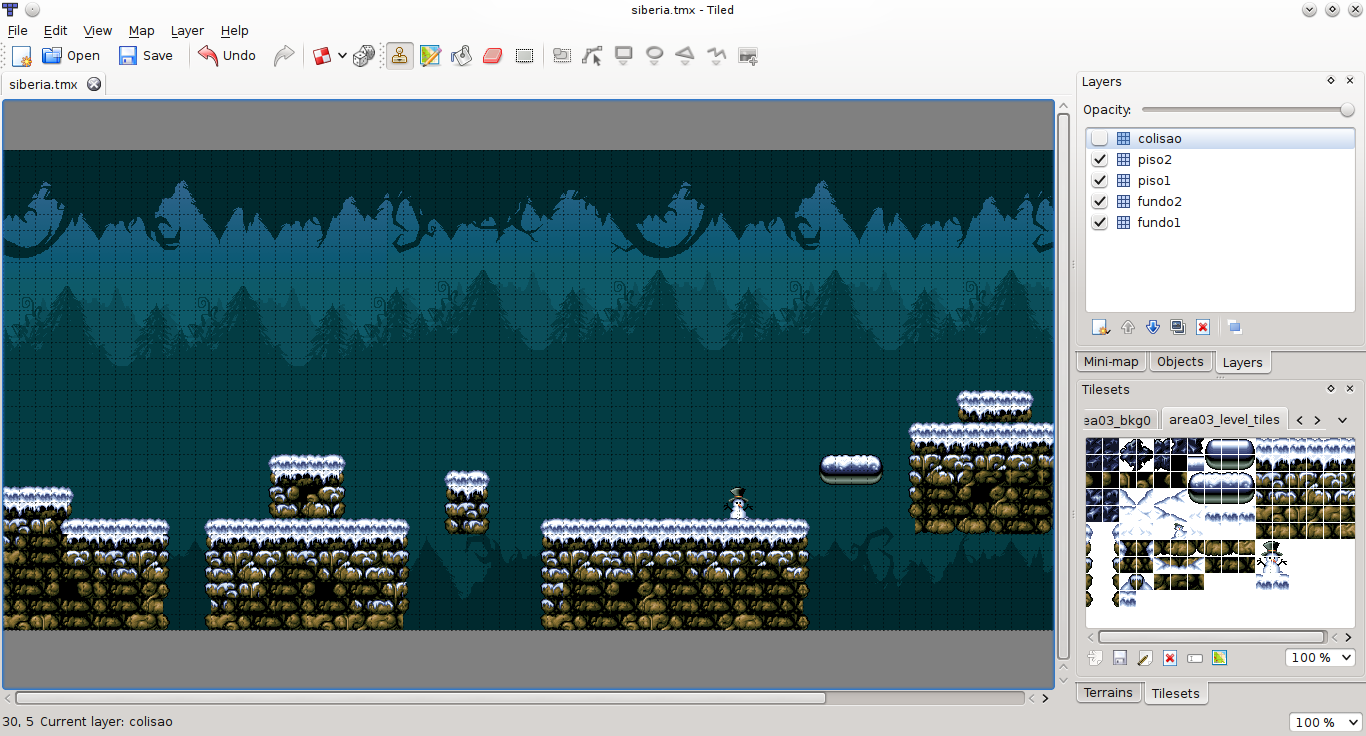
\includegraphics[scale = 0.45]{Imagens/Tiled.png}
    \caption{\textit{Interface do \textit{software} Tiled.}}
    \label{tiled_interface}
\end{figure}
%
\par
Mesmo que o desenvolvedor não queira que seu jogo seja baseado em \textit{tiles}, o software é ainda uma excelente escolha como um editor 
de níveis. Pode-se usá-lo também nas entidades invisíveis, tais como áreas de colisão e o aparecimento de objetos dentro do 
mapa. Por sua simplicidade ela pode ser usada por programadores iniciantes ou experientes.
%
%
%
%
% ----------------------------------------------------------------
% Projeto do sistema *******************
% ----------------------------------------------------------------
\section{Projeto do sistema}
%
Após definido os requisitos do sistema, a próxima etapa foi dar início ao desenvolvimento do projeto. O primeiro passo foi definir, com base nos requisitos e no conhecimento dos envolvidos qual seria a linguagem de programação mais adequada ao problema e qual API deveríamos usar para as rotinas de renderização, leitura dos dispositivos de entrada, reprodução de áudio e etc.
%
%
\subsection{Linguagem de Programação}
\label{linguagem}
%
Até a década de 90 cada jogo tinha a sua \textit{engine}, feita para possibilitar a maior eficiência no uso da memória e da unidade de 
processamento possível, de acordo com as exigências de cada jogo. Um jogo que só usava formas geométricas, por exemplo, não precisava 
tratar imagens na sua \textit{engine}. O nível da microeletrônica e da computação já possibilita o uso de \textit{engines} genéricas, 
mas o desenvolvimento de uma ainda demanda uma programação muito próxima da máquina. 
\par
É por isso que a escolha da linguagem de programação precisa ser feita com cuidado. Considerando o conhecimento da equipe e o propósito do 
projeto, que era uma \textit{engine} didática, para influenciar o designe e o desenvolvimento de jogos de acordo com o nosso alcance, as linguagens de programação selecionadas para a análise foram Actionscript, C++, C\# e Java, de acordo com a simplicidade, o poder e a compatibilidade de cada uma.
%
\subsubsection{Estudo Comparativo}
%
O Actionscript é uma linguagem orientada a objetos desenvolvida pela Macromedia. O que no início era uma ferramenta para controlar animações 
se tornou uma linguagem de script tão complexa que podia ser usada no desenvolvimento de um jogo. Embora essa linguagem ainda seja muito usada 
no desenvolvimento de jogos de web, o que provocou a decisão contrária a ela foi a expectativa de que o HTML 5 viesse a incorporar o Javascript e, 
dessa forma, modificar ou inutilizar o Actionscript.
\par
O C\# (C Sharp) é uma linguagem multi-paradigma da Microsoft feita para o desenvolvimento de sistemas próprios para a plataforma .NET. C\# e Java 
compartilham a mesma simplicidade na leitura e na codificação, assim como a mesma forma de interpretação e compilação, mas um programa em C\# está 
mais próximo da máquina do que um programa em Java. A escolha parecia feita quando nós entendemos que a ligação do C\# com a Microsoft poderia 
custar a compatibilidade do nosso jogo.
\par
Java é uma linguagem orientada a objetos desenvolvida pela Sun, hoje possuída pela Oracle. A sua fama de espaçosa e pesada não é coerente com a 
realidade: hoje a linguagem conta com a Compilação na Hora ou \textit{Just in Time Compilation (JIT Compilation ou só JIT)} , 
para que a sua execução não seja mais interpretada. Mas a sua principal característica é a compatibilidade: a Máquina Virtual do Java ou Java Virtual Machine (JVM) é uma plataforma virtual que pode ser feita compatível para qualquer plataforma física.
\par
Por mais evoluída que seja a JVM, no entanto, o Java não admite o acesso à máquina necessário para o desenvolvimento de uma \textit{game engine}, 
senão com o uso do C++, por meio da Interface Nativa do Java ou Java Native Interface (JNI). Em outras palavras, para usar o Java, nesse caso, 
nós teríamos que usar o C++. Esta, por sua vez, não é a mais simples na codificação, mas não tem limitação alguma tanto em termos de 
compatibilidade quanto em termos de acesso à máquina.
%
\subsubsection{A Escolha: C++}
%
C++ (C Mais Mais ou C Plus Plus) \cite{Novatec} é uma linguagem de programação multi-paradigma, com suporte para a programação imperativa e a programação orientada a objetos, de uso geral, desenvolvida por Bjarne Stroustrup, para formar uma camada de orientação a objetos sobre a linguagem de programação C. O C++ possibilita a programação de baixo nível assim como a programação de alto nível e por isso é considerado uma linguagem de programação de nível médio em termos de proximidade da máquina.
\par
Após o estudo comparativo acima, concluímos que a linguagem C++ seria a melhor opção para o projeto em questão. Tal decisão foi baseada em diversos fatores como experiência e domínio da linguagem pelos envolvidos no projeto, o desempenho das aplicações escritas nesta linguagem e o fato de C++ ser a linguagem de programação mais usada em desenvolvimento de jogos. Uma vez que o objetivo da biblioteca é ser uma porta de entrada para essa área, a escolha da linguagem faz com que o usuário já se familiarize com a mesma. Por último e não menos importante, o C++ é uma linguagem 100\% compatível com a API escolhida como base para a nossa \textit{engine} que será abordada a seguir.
%
%
\subsection{Allegro}
\label{allegro}
%
Nas nossas pesquisas para escolher uma biblioteca com a qual trabalhar, duas se destacaram: a Allegro e a SDL. A SDL (Simple Direct Media Layer - 
Camada de Mídia Direta Simples) é uma popular biblioteca multimídia simples de usar, multiplataforma, de código aberto, e amplamente usada para fazer  jogos e aplicações multimídia. Ela poderia também atender as nossas necessidades, mas a Allegro se destacou por ter um código mais limpo e intuitivo, e rotinas específicas para o desenvolvimento de jogos, como renderização acelerada por hardware e suporte nativos a diversos formatos de imagens e arquivos de áudio. Por esta razão ela foi escolhida.
\par 
Allegro \footnote{Allegro: http://alleg.sourceforge.net/readme.html} é uma biblioteca gráfica multiplataforma, de código fonte aberto e feita na sua maioria em C, mas utilizando internamente também Assembly e C++. Seu nome é um acrônimo recursivo que representa ``\textit{Allegro Low Level Game Routines}'' (``Rotinas de jogo de baixo nível Allegro''). Funciona em diversos compiladores e possui rotinas para a manipulação de funções multimídia de um computador, além de oferecer um ambiente ideal para o desenvolvimento de jogos, tornando-se uma das mais populares ferramentas para esse fim atualmente. Originalmente desenvolvida por Shawn Hargreaves, ela se tornou um projeto colaborativo, com colaboradores de todo o mundo.
\par
Ela possui suporte nativo para rotinas de que utilizam gráficos 2D, embora seja possível utilizá-la em conjuntos com outras API's, como OpenGL e DirectX, para desenvolvimento de aplicações que utilizem gráficos 3D. Apesar de não ser suficiente para o completo desenvolvimento 
de um jogo, existem pequenas bibliotecas adicionais (add-ons), feitas para serem acopladas à Allegro, permitindo assim a sua extensão. Através 
desses add-ons é possível, por exemplo, obter suporte a arquivos MP3, GIF, imagens JPG e vídeos AVI. Isso é útil para que o usuário não tenha que colocar uma porção de funções que não usa na hora de distribuir seu jogo, incluindo somente as partes que for utilizar, diminuindo consideravelmente o tamanho do mesmo.
\par
Atualmente a biblioteca se encontra na sua quinta versão. Allegro 5 foi completamente reescrita e não apresenta compatibilidade com as suas versões anteriores. Foi feito um esforço para tornar a API mais consistente e segura, o que trouxe melhorias funcionais e uma grande mudança na sua arquitetura, sendo agora orientada a eventos e possuindo suporte nativo a aceleração por hardware. Possui a suporte a eventos gerados por dispositivos de entradas como teclado, \textit{mouse} e \textit{joystick} além de funções para desenho de primitivas gráficas, leitura e gravação de seu próprio tipo de arquivo de configuração (muito útil para armazenar configurações e dados de jogos) e é totalmente modular.
\par
A Allegro 5.0 suporta as seguintes plataformas:
%
\begin{itemize}
 \item Windows (MSVC, MinGW);
 \item Unix/Linux;
 \item MacOS X;
 \item iPhone;
 \item Android (Suporte provido pela Allegro 5.1, que ainda se encontra instável).
\end{itemize}
%
A API atualmente se encontra nas versões 5.0.10 (estável) e 5.1.2 (instável). A \textit{SAGA Game Library} foi desenvolvida usando como base a versão 5.0.10, por a mesma ser estável.
%
\subsubsection{Principais Recursos e Funções}
%
A seguir, encontramos um conjunto dos principais recursos da Allegro 5, começando com as funções mais gerais da biblioteca.
%
\begin{itemize}
 \item \textbf{al\_init()}: Inicializa a biblioteca Allegro, dando valores a algumas variáveis globais e reservando memória. 
 Deve ser a primeira função a ser chamada.
 \item \textbf{al\_exit()}: Encerra a Allegro. Isto inclui retornar ao modo texto e remover qualquer rotina que tenha sido instalada. 
 Não há necessidade de chamar essa função explicitamente, pois, normalmente, isto é feito quando o programa termina.
\end{itemize}
%
As rotinas de vídeo:
%
\begin{itemize}
 \item \textbf{ALLEGRO\_DISPLAY}: Tipo que representa a janela principal. A biblioteca permite que se trabalhe com múltiplas janelas.
 \item \textbf{al\_create\_display(width, height)}: Cria uma instância da janela, retornando um ponteiro para ALLEGRO\_DISPLAY. 
 Os parâmetros indicam as dimensões em pixels.
 \item \textbf{al\_flip\_display()}: Função para atualizar a tela.
 \item \textbf{al\_destroy\_display(var)}: Finaliza a instância \textit{var} do tipo ALLEGRO\_DISPLAY\*.
\end{itemize}
%
As rotinas para manipulação de arquivos de imagem:
%
\begin{itemize}
 \item \textbf{ALLEGRO\_BITMAP}: Tipo que representa o arquivo de imagem carregado pela Allegro.
 \item \textbf{al\_init\_image\_addon()}: Inicializa o add-on da Allegro 5 para utilização de imagens.
 \item \textbf{al\_load\_bitmap(``example.jpg'')}: Carrega a imagem indicando no parâmetro o nome e tipo. Ela deve estar previamente salva na pasta 
 do programa. Recebe o caminho relativo ou absoluto da imagem a ser carregada, retornando um ponteiro para o tipo ALLEGRO\_BITMAP.
 \item \textbf{al\_draw\_bitmap(bitmap, x, y, mirror)}: Função para desenhar a imagem na tela. Os parâmetros são o bitmap a ser desenhado, as 
 posições x e y e as flags de espelhamento (0, ALLEGRO\_FLIP\_HORIZONTAL, ALLEGRO\_FLIP\_VERTICAL).
\end{itemize}
% 
As rotinas de áudio:
%
\begin{itemize}
 \item \textbf{ALLEGRO\_SAMPLE}: Tipo que representa arquivos pequenos, geralmente efeitos sonoros.
 \item \textbf{ALLEGRO\_AUDIO\_STREAM}: Tipo para representar arquivos grandes, de forma que o arquivo não é carregado de uma vez para a 
 memória. Geralmente representa os arquivos que irão compor uma trilha sonora.
 \item \textbf{al\_install\_audio()} e \textbf{al\_init\_acodec\_addon()}: A primeira inicializa as funções relativas ao áudio. A segunda inicializa os 
 codecs necessários para carregar os diversos formatos de arquivo suportados. Fornece suporte a alguns formatos, como Ogg, Flac e Wave.
 \item \textbf{al\_set\_audio\_stream\_playing(musica, true)}: Função que recebe o arquivo de áudio já carregado no primeiro parâmetro e um tipo 
 booleano no segundo (true para fazê-la tocar ou false, em caso contrário).
 \item \textbf{al\_destroy\_audio\_stream(musica) } e \textbf{al\_destroy\_sample(sample)}: Funções de desalocação dos arquivo de áudio carregados 
 pela Allegro.
\end{itemize}
%
%
A Allegro ainda possui muitos recursos que não foram citados devido a sua quantidade. Posteriormente, a API será explorada mais a fundo conforme os recursos da \textit{SAGA Game Library} forem sendo mostrados.
%
%
\subsection{Suporte ao Tiled}
%
O Tiled faz a edição de várias camadas de \textit{tiles} e salva tudo em um formato padronizado de extensão ``.tmx''. Uma das principais vantagens do formato TMX é sua organização, detalhamento e praticidade, sendo que seu conteúdo pode ser lido através do uso de um \textit{parser} para arquivos XML.
\par 
Existem inúmeros \textit{parsers} de arquivos XML, cada um com suas vantagens e desvantagens. Entre os \textit{parser} mais populares podemos citar a RapidXML e a TinyXML. Segundos comparação do próprio desenvolvedor, a RapidXML apresenta a maior velocidade da leitura de dados entre os \textit{parsers} as mais populares mas o escolhido foi a TinyXML, por sua simplicidade de uso e velocidade que não apresenta uma diferença significativa a sua concorrente RapiXML. 
%
%
\subsubsection{A biblioteca TinyXML}
\label{tinyXML}
%
É uma biblioteca escrita em C++ que analisa uma sequência de entrada no formato XML permitindo o acesso aos dados contidos nesse último. Em outras palavras, ela realiza o \textit{parser} de uma arquivo .xml e armazena a informação em objetos C++ que podem ser manipulados livremente. 
\par 
A TinyXML \footnote{http://www.grinninglizard.com/tinyxml/} pode ser facilmente integrada em outros programas, bastando apenas adicionar seus 
arquivos ao projeto. Com ela é possível realizar o acesso aos dados direta ou iterativamente, alteração da estrutura através 
de inserção e remoção de elementos, remoção de espaços duplicados e a gravação para ficheiros em formato XML.
TinyXML é uma estrutura extremamente compacta e robusta, elaborada para um rápido e fácil aprendizado. Pode ser usada para 
fins de código aberto ou comerciais. Ela é compatível com UTF-8, de modo a permitir que arquivos XML sejam manipulados em 
qualquer linguagem. Também apresenta grande simplicidade em seu uso e rapidez na leitura de dados.
%
%
\subsubsection{Tiled: Codificação e compactação de dados}
%
%
Um dos recursos mais interessantes do Tiled é a possibilita de exportar os dados contidos no arquivo .tmx de forma compactada e codificação. 
A principal vantagem do uso dos algoritmos compactação e codificação é a redução do tamanho em disco do arquivo .tmx resultante e aumento da velocidade de carregamento do cenário, uma vez que a biblioteca carrega os dados codificados e/ou compactados e os decodifica/descompacta a nível de software ao invés de realizar a leitura dos mesmo em disco. 
\par 
A compactação de dados fornecida pelo Tiled é realizada pelas bibliotecas ZLIB \footnote{ZLIB: http://www.zlib.net/} e GZIP \footnote{GZIP: http://www.gnu.org/software/gzip/gzip.html}, enquanto a codificação é realizada pelo algoritmo Base64 fornecido por \footnote{Algoritmo Base64: http://www.adp-gmbh.ch/cpp/common/base64.html}, também fornecido por uma biblioteca externa.
São fornecidas as opções de exportar os dados no arquivo .tmx na forma codificada e compactada ou apenas na forma codificada. Também são oferecidas as opções de exportar os dados em formato puro (sem codificação) XML ou no formato CVS. 
\par 
A seguir podemos verificar a redução do tamanho em disco de um arquivo .tmx em relação ao seu tamanho em disco sem codificação/compactação.
%
\begin{itemize}
 \item Arquivo XML puro( sem codificação/compactação): 31,3 KB;
 \item Com codificação Base64: 9,6 KB;
 \item Com codificação Base64 e compressão GZIP: 2,2 KB;
 \item Com codificação Base64 e compressão ZLIB: 2,1 KB;
 \item No formato CVS: 4,9 KB.
\end{itemize}
%
A \textit{SAGA Game Library} prove suporte total e otimizado as 5 opções de exportação acima. Ela, assim com o Tiled, também faz
uso das bibliotecas GZIP e ZLIB para descompactação e também realiza a decodificação dos dados em Base64 contidos no arquivo .tmx (detalhes de uso serão abordados posteriormente).
%
%
%
%
% ----------------------------------------------------------------
% Implementação *******************
% ----------------------------------------------------------------
\section{Implementação da biblioteca}
%
%
A \textit{SAGA Game Library} é uma \textit{engine} orientada a objeto desenvolvida em C++ sobre a API Allegro 5. Ela possui todos os recursos que uma \textit{engine} básica possui, como suporte a criação de \textit{sprites} animados e estáticos, criação de cenários usando o editor de níveis Tiled, suporte ao uso de fontes de texto TTF e a diversos formatos de arquivos de áudio. Também possui gerenciamento de automático de recursos (imagem, fontes e áudio), o que possibilita economia significativa de memória. A biblioteca fornece uma estrutura para implementação do \textit{game loop} e suporte para eventos de teclado, \textit{mouse} e \textit{joystick} também estão presentes. 
\par 
Após a fase de projeto, deu-se sequência a fase de estudo do problema. Está fase resumiu-se simplesmente no estudo do problema a fim de torná-lo orientado a objetos. Internamente, a \textit{SAGA Game Library} consiste em um \textit{package} denominado \textit{sgl} e subdivididas em 4 outros \textit{packages} com funções específicas: \textit{image, font, audio e input}.
%
%
\begin{itemize}
 \item image: consiste nas classe exclusivamente relacionadas a parte gráfica da \textit{engine}, o que inclui manipulação de arquivos de imagens como \textit{sprites} animados e estáticos e carregamento e renderização de cenários do jogo;
 \item font: é o responsável pela parte textual da biblioteca. Ele carrega uma fonte no formato TTF (``True Type Font'') padrão do Windows e a utiliza para escrever textos na tela de jogo;
 \item audio: \textit{package} destinado ao carregamento, manuseio e reprodução dos arquivos de áudio;
 \item input: incluí todas as funções relacionadas aos comandos recebidos pelos dispositivos de entradas do computador (teclado, \textit{mouse} e \textit{joystick}).
\end{itemize}
%
Abaixo podemos visualizar o esquema da organização da \textit{engine}. A seguir, serão abordados os principais recursos da biblioteca bem como os detalhes da suas respectivas implementações.
%
%
%
%
\begin{figure}[H]
    \centering
    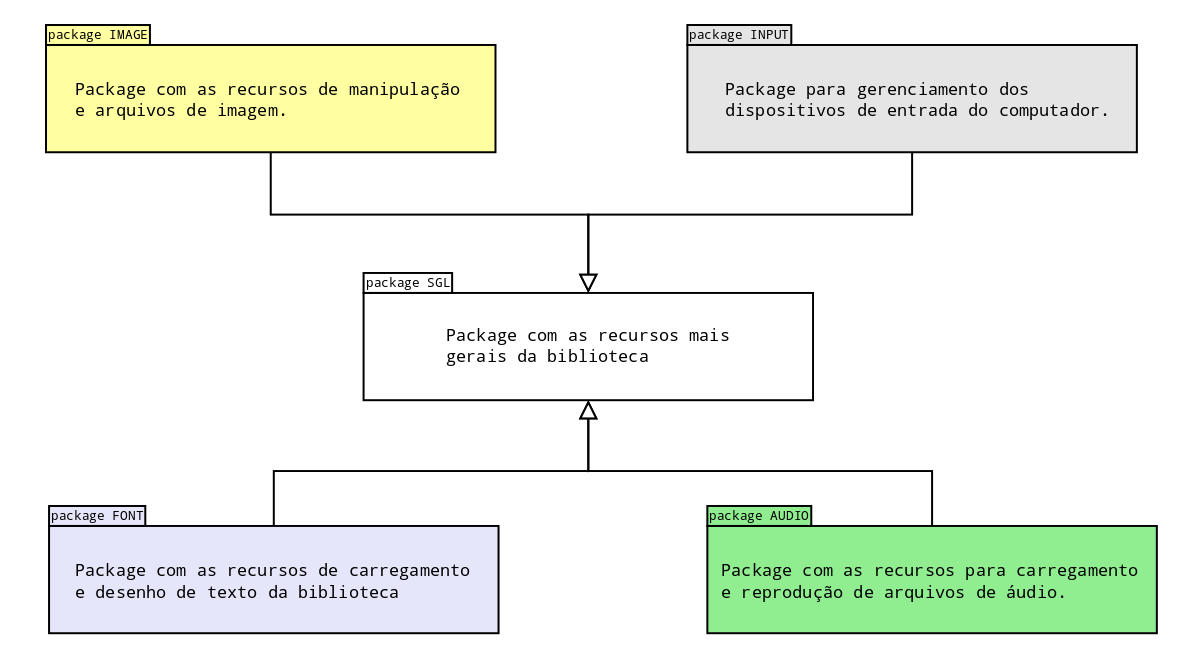
\includegraphics[scale = 0.2]{Imagens/pacotes.png}
    \caption{Esquema estrutural da SGL.}
    \label{pacotes}
\end{figure}
%
%
%
\subsection{SGL}
%
%
É o pacote mais geral, e que engloba todos os outros. Quando a funcionalidade de uma classe não é específica ou é usada como ferramenta auxiliar em outras classes, ela é colocada nesse pacote.
%
\subsubsection{AllegroStarter}
%
Cada um dos módulos da Allegro deve ser inicializado antes de seu uso. A Classe AllegroStarter é responsável e também por desalocar os recursos quando o programa é fechado. Uma exceção é lançada caso algum dispositivo apresente problemas durante a inicialização. Também contém informações sobre a atual versão da Allegro. 
%
%
\subsubsection{SGLException}
%
É a classe que captura e trata as exceções que possam ocorrer durante a execução do programa, como inicialização dos componentes da allegro e carregamento de arquivos de imagem, fonte e áudio. A classe é uma especialização de std::exception. Abaixo temos um exemplo de uso desta classe.
%
\lstinputlisting{CodigoFonte/ExemploSGLException.cpp}
%
\par 
Caso ocorra algum erro de inicialização da Allegro, a função \textit{al\_init()} retornará \textit{false}, fazendo com que o programa execute o conteúdo do \textit{if} e lance a exceção. No console, teremos a mensagem:  ``\textit{terminate called after throwing an instance of `sgl::Exception'
what(): Failed to initialize ALLEGRO\_Lib.}''.
%
%
\subsubsection{Color}
%
%
A classe Color possui recursos para trabalharmos com diversos formatos de especificação de cores, como RGB e HTML. Os objetos dessa classe podem ser usadas, por exemplo, para colorir a tela ou alterar a cor de uma determinada fonte de texto. Ela aceita dois construtores. Com o primeiro deles é possível definir cores no formato RGB. Para isso, o construtor recebe três parâmetros que variam de 0 a 255, um para vermelho, outro para verde e outro para azul, respectivamente. O segundo construtor aceita strings no formato html ou o nome em inglês de uma cor, desde que ele já esteja pré-definido. Alguns dos nomes válidos são: \textit{cyan}, \textit{lightgreen}, \textit{green} entre outros. Caso o nome de uma cor inexistente seja passado como parâmentro, o contrutor cria um objeto com as coordenadas RGB iguais a 0 (cor preta). A seguir temos alguns exemplos de uso da classe Color.
%
%
\lstinputlisting{CodigoFonte/ExemploColor.cpp}
%
%
\subsubsection{Video}
%
%
Classe responsável por gerenciar todos os recursos de vídeo da \textit{engine}. Através dela, tem-se acesso a todas as rotinas pertinentes (de atualização de tela, posicionamento, e outros eventos) para o gerenciamento de vídeo. A classe também possibilita a escolha por parte do usuário de criar um \textit{display} no formato de janela ou em \textit{fullscreen}, e também permite a escolha de uma API para renderização 3D, como OpenGL (Linux e Windows) e DirectX (Windows). 
\par 
Quando criarmos um objeto da classe Video, devemos definir as dimensões do \textit{display}, dado pelas coordenadas x e y conforme o desenho e o modo (WINDOWED, FULLSCREEN) no construtor da classe. Por padrão, a cor de fundo do vídeo é preta, podendo ser alterada. Também existe a possibilidade de adicionar um ícone e um título para nossa janela. A função \textit{refresh()} é responsável por por transferir o conteúdo da memória de vídeo para o \textit{display} e deve ser chamada sempre que seja necessário atualizar o \textit{display}, caso contrário, nenhum das ações realizadas pelas rotinas de desenho serão visualizadas. 
\par 
A principal dificuldade na implementação da classe foi aprender como a Allegro fazia uso da memória de vídeo e dos conceitos envolvidos como taxa de atualização do \textit{display}, uso do \textit{vsync} e de como poderíamos tirar o máximo proveito disso. O principal fator foi quanto ao desempenho da renderização da tela. Isso foi resolvido ajustando a Allegro para que a mesma armazena-se todos as imagens a serem desenhadas na memória de vídeo ao invés da memória RAM. Essa configuração apresentou resultados significativos no uso do processador. Enquanto as imagens armazenadas na RAM utilizavam 25\% da CPU, as mesmas imagens armazenadas na memória de vídeo não consumiam mais de 2\% do processador durante o processo de desenho no \textit{display}.
\par
A seguir temos a classe Video em detalhes.
%
%
%
%
\begin{figure}[H]
    \centering
    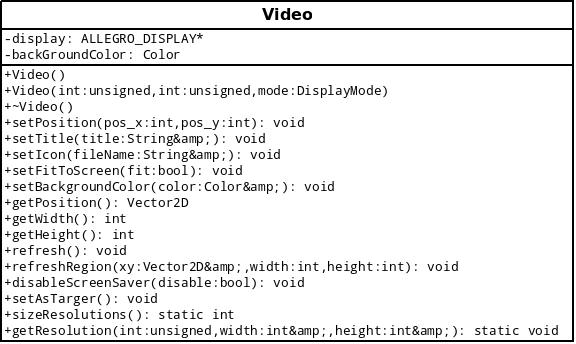
\includegraphics[scale = 0.5]{uml/video.jpeg}
    \caption{UML da classe Video.}
    \label{umlVideo}
\end{figure}
%
%
e um exemplo de uso da mesma.
%
%
\lstinputlisting{CodigoFonte/ExemploDisplay.cpp}
%
%
\begin{figure}[H]
    \centering
    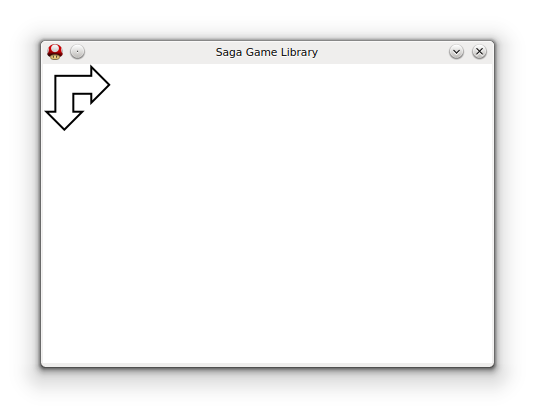
\includegraphics[scale = 0.8]{Imagens/display.png}
    \caption{Display criado com o uso da classe Video.}
    \label{display}
\end{figure}
%
%
\subsubsection{Vector2D}
%
%
A classe Vector2D é uma das classe mais importantes da \textit{SAGA Game LIbrary}. A classe Vector2D tal qual o nome diz, define um vetor bidimensional, iniciando-se no ponto (0,0) da tela e indo até o ponto (x,y) definido pelo usuário, sendo responsável pelo posicionamento de qualquer entidade, seja ela um \textit{sprite} ou um texto, no \textit{display}. A escolha do uso de vetores ao invés de simples coordenadas deve-se a vantagens que o uso de vetores oferece. Muitas operações matemáticas como deslocamento, rotações e escalonamentos são feitas utilizando vetores. Até mesmo efeitos de física, como gravidade e aceleração são executados usando como base os conceitos de mecânica clássica. A vantagem do vetor sobre um par de coordenadas (x,y) deve-se a quantidade de informação que o primeiro carrega. Enquanto um ponto representa apenas uma localização no espaço, um vetor possui uma direção, sentido e magnitude. 
\par 
Assim como ocorre na geometria, os vetores também possibilitam diversas operações algébricas entre eles, através da sobrecarga de operadores. Soma e subtração de vetores, normalização são algumas das operações possíveis e que podem ser usadas para se obter interessantes resultados, como uma simulação de gravidade ilustrada na figura abaixo, onde temos um vetor representando o deslocamento do personagem e outro representando a força gravitacional.
%
%
%
\begin{figure}[H]
    \centering
    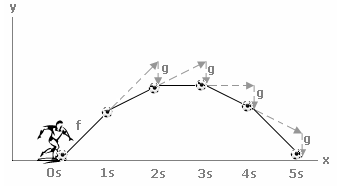
\includegraphics[scale = 0.8]{Imagens/VetorGravidade.png}
    \caption{Uso de vetores na simulação de gravidade.}
    \label{VetorGravidade}
\end{figure}
%
%
%


